\section{Auswertung}
\label{sec:Auswertung}

Für die Auswertung wird Python, im Speziellen matplotlib \cite{matplotlib}, 
SciPy \cite{scipy}, Uncertainties \cite{uncertainties}
und NumPy \cite{numpy} benutzt.

\subsection{Elektisches Feld}
\subsubsection{Proportionalität zwischen Leuchtfleckverschiebung und Ablenkspannung}
\label{sec:prop}
%Tabellen
Die gemessenen Werte für die Ablenkspannung $U_\text{d}$
auf jeder Linie des Koordinatennetzes sind für die fünf
unterschiedlichen Beschleunigungsspannungen $U_\text{B}$
in den folgenden Tabellen \ref{taba1} bis \ref{taba5} aufgelistet.
\begin{table}\caption{Der magnetische Fluss $B$ an verschiedenen Stellen $x$ in der langen Spule.}
\label{taba1}
\centering
\sisetup{round-mode = places, round-precision=3, round-integer-to-decimal=true}
\begin{tabular}{S[]S[]} 
\toprule
{$B$/ \si{\milli\tesla}} & {$x$/ \si{\centi\meter}}\\
\midrule
0.382 & 0.0\\
0.505 & 0.5\\
0.744 & 1.0\\
0.959 & 1.5\\
1.35 & 2.0\\
1.544 & 2.5\\
1.7619999999999998 & 3.0\\
1.928 & 3.5000000000000004\\
2.024 & 4.0\\
2.093 & 4.5\\
2.1380000000000003 & 5.0\\
2.173 & 5.5\\
2.2030000000000003 & 6.0\\
2.2239999999999998 & 6.5\\
2.238 & 7.000000000000001\\
2.248 & 7.5\\
2.2560000000000002 & 8.0\\
2.262 & 8.5\\
2.265 & 9.0\\
2.2659999999999996 & 9.5\\
2.264 & 10.0\\
2.2560000000000002 & 10.5\\
2.2520000000000002 & 11.0\\
2.247 & 11.5\\
2.241 & 12.0\\
2.231 & 12.5\\
2.219 & 13.0\\
2.221 & 13.5\\
2.222 & 14.000000000000002\\
2.22 & 14.499999999999998\\
2.216 & 15.0\\
2.212 & 15.5\\
2.238 & 16.0\\
2.245 & 16.5\\
2.2230000000000003 & 17.0\\
2.209 & 17.5\\
2.1870000000000003 & 18.0\\
2.1519999999999997 & 18.5\\
2.088 & 19.0\\
2.0 & 19.5\\
1.874 & 20.0\\
1.673 & 20.5\\
1.4469999999999998 & 21.0\\
1.1509999999999998 & 21.5\\
0.82 & 22.0\\
0.575 & 22.5\\
0.416 & 23.0\\
0.303 & 23.5\\
0.221 & 24.0\\
\bottomrule
\end{tabular}\end{table}
\begin{table}\caption{Die Index Werte entsprechen der Höhe, die bei der jeweiligen Ablenkspannung $U_\text{d}$ und der Beschleunigungsspannung $U_\text{B} = \SI{230}{\volt}$ gemessen wurden. Der Indexwert $1$ entspricht einer Höhe von $\SI{0.6}{\centi\meter}$.}
\label{taba2}
\centering
\sisetup{round-mode = places, round-precision=1, round-integer-to-decimal=true}
\begin{tabular}{S[]S[]} 
\toprule
{Index} & {$U_\text{d} / \si{\volt}$}\\
\midrule
1.0 & -25.8\\
2.0 & -21.8\\
3.0 & -17.8\\
4.0 & -13.5\\
5.0 & -9.4\\
6.0 & -5.2\\
7.0 & -1.0\\
8.0 & 3.4\\
9.0 & 7.8\\
\bottomrule
\end{tabular}\end{table}
\begin{table}\caption{Die Indexwerte entsprechen der Höhe, die bei der jeweiligen Ablenkspannung $U_\text{d}$ und der Beschleunigungsspannung $U_\text{B} = \SI{280}{\volt}$ gemessen wurden. Der Indexwert $1$ entspricht einer Höhe von $\SI{0.6}{\centi\meter}$.}
\label{taba3}
\centering
\sisetup{round-mode = places, round-precision=1, round-integer-to-decimal=true}
\begin{tabular}{S[]S[]} 
\toprule
{Index} & {$U_\text{d} / \si{\volt}$}\\
\midrule
1.0 & -30.7\\
2.0 & -26.0\\
3.0 & -20.8\\
4.0 & -15.9\\
5.0 & -10.9\\
6.0 & -5.8\\
7.0 & -0.9\\
8.0 & 4.6\\
9.0 & 10.0\\
\bottomrule
\end{tabular}\end{table}
\begin{table}\caption{Die Index Werte entsprechen der Höhe die bei der jeweiligen Ablenkspannung $U_d$ und der Beschleunigungsspannung $U_\text{B} = \SI{330}{\volt}$.}
\label{taba4}
\centering
\sisetup{round-mode = places, round-precision=1, round-integer-to-decimal=true}
\begin{tabular}{S[]S[]} 
\toprule
{Index} & {$U_\text{d} / \si{\volt}$}\\
\midrule
1.0 & -36.1\\
2.0 & -30.1\\
3.0 & -24.4\\
4.0 & -18.3\\
5.0 & -12.6\\
6.0 & -6.8\\
7.0 & -0.6\\
8.0 & 5.7\\
9.0 & 12.1\\
\bottomrule
\end{tabular}\end{table}
\begin{table}\caption{Die Index Werte entsprechen der Höhe, die bei der jeweiligen Ablenkspannung $U_\text{d}$ und der Beschleunigungsspannung $U_\text{B} = \SI{380}{\volt}$ gemessen wurden. Der Indexwert $1$ entspricht einer Höhe von $\SI{0.6}{\centi\meter}$.}
\label{taba5}
\centering
\sisetup{round-mode = places, round-precision=1, round-integer-to-decimal=true}
\begin{tabular}{S[]S[]} 
\toprule
{Index} & {$U_\text{d} / \si{\volt}$}\\
\midrule
1.0 & nan\\
2.0 & -34.6\\
3.0 & -27.7\\
4.0 & -21.0\\
5.0 & -14.3\\
6.0 & -7.5\\
7.0 & -0.4\\
8.0 & 6.8\\
9.0 & 13.6\\
\bottomrule
\end{tabular}\end{table}

%D gegen U_d (plot1) -> D/U_d für verschiedene U_B
\noindent Die Leuchtfleckverschiebung $D$ ist in Tab. \ref{tab1} und in Abb. \ref{fig:plot1}
für die fünf Beschleunigungsspannungen gegen das Verhältnis aus 
Ablenkspannung $U_\text{d}$ und der Beschleunigungsspannung $U_\text{B}$ aufgetragen.

\begin{table}\caption{Der maximale Drehimpuls $L$, der Gesamtspin $S$ und der Gesamtdrehimpuls $J$ ergeben sich zum Landé-Faktor $g_\text{J}$ für die vier verschiedenen Elemente.}
\label{tab1}
\centering
\sisetup{round-mode = places, round-precision=2, round-integer-to-decimal=true}
\begin{tabular}{S[]S[]S[]S[]} 
\toprule
{$L$} & {$S$} & {$J$} & {$g_\text{J}$}\\
\midrule
5.0 & 1.0 & 4.0 & 0.8\\
0.0 & 3.5 & 3.5 & 2.0\\
6.0 & 1.5 & 4.5 & 0.7272727272727273\\
5.0 & 2.5 & 7.5 & 1.3333333333333333\\
\bottomrule
\end{tabular}\end{table}

\begin{figure}
    \centering
    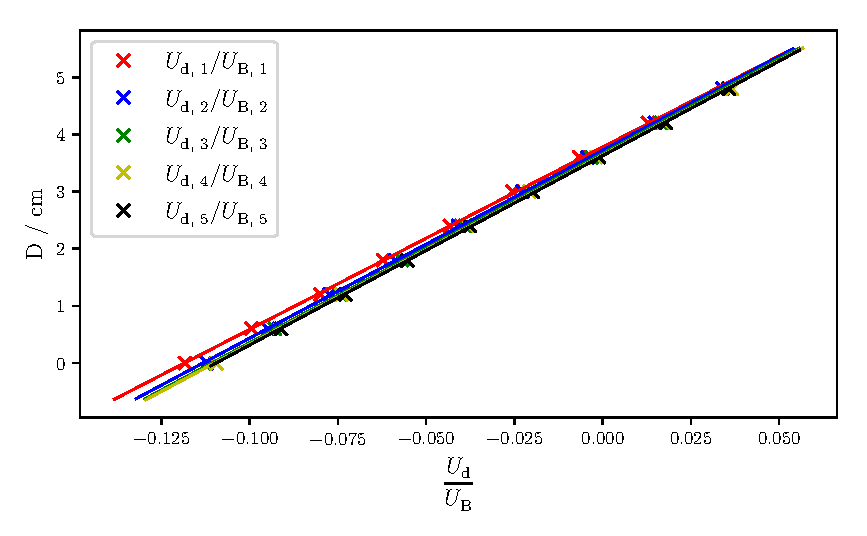
\includegraphics[width=12cm, height=7cm]{build/plot1.pdf}
    \caption{Die Leuchtfleckverschiebung $D$ ist gegen das Verhältnis aus 
        Ablenkspannung $U_\text{d}$ und die Beschleunigungsspannung $U_\text{B}$ aufgetragen. Es sind die Daten
    für die fünf verschiedenen Beschleunigungsspannungen und
    jeweils einen Fit eingezeichnet.}
    \label{fig:plot1}
\end{figure}

\noindent Aus dem Fit in Abb. \ref{fig:plot1} lässt sich die Steigung  
$\frac{p L}{2 d}$ experimentell bestimmen:
\begin{align*} 
   U_\text{B} = \SI{180}{\volt} \Rightarrow \frac{p L}{2 d} &= \SI{31.88(22)}{\centi\meter\per\volt} \\
    U_\text{B} = \SI{230}{\volt} \Rightarrow \frac{p L}{2 d} &= \SI{32.86(18)}{\centi\meter\per\volt} \\
    U_\text{B} = \SI{280}{\volt} \Rightarrow \frac{p L}{2 d} &= \SI{33.09(22)}{\centi\meter\per\volt} \\
    U_\text{B} = \SI{330}{\volt} \Rightarrow \frac{p L}{2 d} &= \SI{33.05(22)}{\centi\meter\per\volt} \\
    U_\text{B} = \SI{380}{\volt} \Rightarrow \frac{p L}{2 d} &= \SI{33.10(15)}{\centi\meter\per\volt}.
\end{align*} %das sieht hässlich aus, weiß nicht wie man das machen könnte
Der mit Gleichung %Gleichung Mittelwert
errechnete Mittelwert für die Steigung ist
\begin{equation*}
    \frac{D}{U_\text{D}} = \SI{32.8(5)}{\centi\meter\per\volt}.
\end{equation*}

%Werte p, d, L angeben
\noindent Die angegebenen Werte für die Plattenlänge $p$,
den Plattenabstand $d$ und den Strahlweg $L$ sind
\begin{align*}
    p &= \SI{1.03}{\centi\meter} \\
    d &= \SI{0.38}{\centi\meter} \\
    L &= \SI{14.3}{\centi\meter}.
\end{align*}

%pL/2d mit a vergleichen
Der aus diesen Werten theoretisch berechnete Wert für die
Steigung ist
\begin{equation*}
    \frac{p \, L}{2 \, d} = \SI{19.38}{\centi\meter}.
\end{equation*}

\subsubsection{Bestimmung der Frequenz der Sinusspannung}
Die gemessenen Synchronisationsfrequenzen sind in Tabelle
\ref{tabb} zu finden. 
\begin{table}\caption{Die angelegte Spannung des elektrischen Feldes innerhalb des Geiger-Müller-Zählrohrs, die Anzahl der jeweils gemessenen Impulse und der Strom innerhalb des Geiger-Müller-Zählrohrs.}
\label{tabb}
\centering
\sisetup{round-mode = places, round-precision=2, round-integer-to-decimal=true}
\begin{tabular}{c c S[]} 
\toprule
{$U / \si{\volt}$} & {$\frac{N}{\SI{130}{\second}}$} & {$I / \si{\ampere}$}\\
\midrule
320 & 11298 & 0.1\\
400 & 11820 & 0.2\\
480 & 12135 & 0.3\\
540 & 12301 & 0.35\\
560 & 12068 & 0.4\\
600 & 12354 & 0.45\\
640 & 12403 & 0.5\\
660 & 12507 & 0.55\\
680 & 12659 & 0.6\\
\bottomrule
\end{tabular}\end{table}

%v_Sinus
\noindent Durch das Synchronisationsverhältnis
%Gleichung Verhältnis
kann jeweils die Frequenz der Sinusspannung bestimmt werden:
\begin{align*}
    \nu_1 &= \SI{50.04}{\hertz} \\
    \nu_2 &= \SI{49.95}{\hertz} \\
    \nu_3 &= \SI{49.995}{\hertz} \\
    \nu_4 &= \SI{49.99}{\hertz}.
\end{align*}
Der daraus mit Gleichung
%Gleichung Mittelwert
berechnete Mittelwert ergibt sich zu
\begin{equation*}
    \nu_\text{mittel} = \SI{49.994(32)}{\hertz}.
\end{equation*}


\subsection{Magnetfeld}
\subsubsection{Bestimmung der spezifischen Elektronenladung}
Die Strahlverschiebung $D$ in Abhängigkeit von der Flussdichte $B$
für eine Beschleunigungsspannung von $U_\text{B} = \SI{250}{\volt}$
ist in Tabelle \ref{tabc1} aufgeführt. Die Strahlverschiebung in
Abhängigkeit von der Flussdichte für eine Beschleunigungsspannung
von $U_\text{B} = \SI{360}{\volt}$ befindet sich in Tabelle \ref{tabc2}.
\begin{table}\caption{Die Indexwerte entsprechen der Höhe bei dem jeweiligen Strom und der Beschleunigungsspannung $U_\text{B} = \SI{250}{\volt}$.}
\label{tabc1}
\centering
\sisetup{round-mode = places, round-precision=2, round-integer-to-decimal=true}
\begin{tabular}{S[]S[]} 
\toprule
{Index} & {$I / \si{\ampere}$}\\
\midrule
1.0 & 0.0\\
2.0 & 0.25\\
3.0 & 0.625\\
4.0 & 1.0\\
5.0 & 1.35\\
6.0 & 1.675\\
7.0 & 2.05\\
8.0 & 2.4\\
9.0 & 2.75\\
\bottomrule
\end{tabular}\end{table}
\begin{table}\caption{Die Indexwerte entsprechen der Höhe bei dem jeweiligen Strom und der Beschleunigungsspannung $U_\text{B} = \SI{360}{\volt}$.}
\label{tabc2}
\centering
\sisetup{round-mode = places, round-precision=2, round-integer-to-decimal=true}
\begin{tabular}{S[]S[]} 
\toprule
{Index} & {$I / \si{\ampere}$}\\
\midrule
1.0 & 0.0\\
2.0 & 0.325\\
3.0 & 0.75\\
4.0 & 1.175\\
5.0 & 1.55\\
6.0 & 1.95\\
7.0 & 2.375\\
8.0 & 2.8\\
9.0 & 3.225\\
\bottomrule
\end{tabular}\end{table}

%D/(L^2+D^2) gegen B (plot 2) für beide U_B -> Faktor a -> e_0/m_0
%Weg L angeben
\noindent Der Term $\frac{D}{L^2 + D^2}$ ist für beide Beschleunigungsspannungen
in Tab. \ref{tab2} Abb. \ref{fig:plot2} aufgetragen. Dabei ist $L$ der Strahlweg und
hat einen Wert von
\begin{equation*}
    L = \SI{14.3}{\centi\meter},
\end{equation*}
wie bereits in Abschnitt \ref{sec:prop} erwähnt.

\begin{table}\caption{Das Verhältnis des magnetischen Feldes durch die Beschleunigungsspannung aufgetragen gegen die Höhe.}
\label{tab2}
\centering
\sisetup{round-mode = places, round-precision=2, round-integer-to-decimal=true}
\begin{tabular}{S[]S[]S[]} 
\toprule
{$B_1 / \si{\henry}$} & {$B_2 / \si{\henry}$} & {$\frac{D}{(L^2 + D^2)} / \si{\per\meter}$}\\
\midrule
0.0 & 0.0 & 0.0\\
3.5649278338607584e-07 & 3.862005153349155e-07 & 0.29289724188430566\\
8.912319584651897e-07 & 8.912319584651897e-07 & 0.5827222842713544\\
1.4259711335443034e-06 & 1.396263401595464e-06 & 0.8665094112549946\\
1.9250610302848096e-06 & 1.8418793808280586e-06 & 1.1414982164090373\\
2.3885016486867084e-06 & 2.3172030920094934e-06 & 1.4052180429996723\\
2.923240823765822e-06 & 2.822234535139767e-06 & 1.6555530006898145\\
3.4223307205063282e-06 & 3.3272659782700412e-06 & 1.8907846756403912\\
\bottomrule
\end{tabular}\end{table}

\begin{figure}
    \centering
    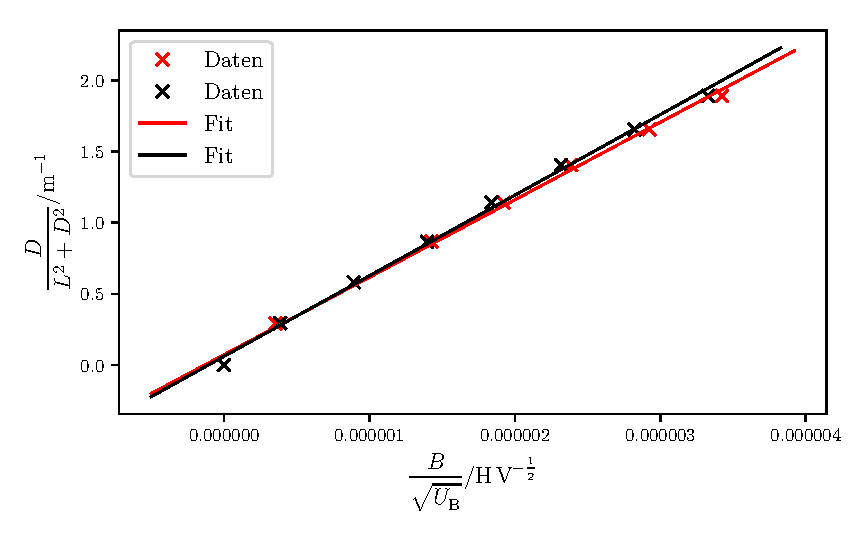
\includegraphics[width=12cm, height=7cm]{build/plot2.pdf}
    \caption{$\frac{D}{L^2 + D^2}$ gegen $\frac{B}{\sqrt{8 U_\text{B}}}$ aufgetragen.
    Es sind die Daten und die Fits für beide Beschleunigungsspannungen
    eingetragen.}
    \label{fig:plot2}
\end{figure}

\noindent Durch die quadrierte Steigung der beiden Fits
lässt sich die spezifische Elektronenladung experimentell bestimmen.
Diese ergibt sich zu
\begin{equation*}
    \frac{e_0}{m_0} = \SI{3.09(12)e11}{\coulomb\per\kilogram}.
\end{equation*}

Der Literaturwert liegt bei 
\begin{equation*}
    \frac{e_0}{m_0} = \SI{<++>}{\coulomb\per\kilo\gram}.
\end{equation*}

\subsubsection{Bestimmung der Intensität des lokal Erdmagnetfelds}
%Werte I_hor und phi angeben -> B_total
Der Spulenstrom, der nötig ist, um das Erdmagnetfeld zu
kompensieren, beträgt
\begin{equation*}
    I_\text{hor} = \SI{0.19}{\ampere}.
\end{equation*}
Der Winkel zwischen Horizontalebene und Richtung des Erdmagnetfelds
beträgt
\begin{equation*}
    \varphi = \SI{79.5}{\degree}.
\end{equation*}
Aus diesen beiden Werten lässt sich mittels Gleichung %Gleichung B_total
die Totalintensität des lokalen Erdmagnetfelds bestimmen.
Diese ergibt sich zu
\begin{equation*}
    B_\text{total} = \SI{6.65e-5}{\tesla}.
\end{equation*}
